\chapter{Background Material}
The aim of this chapter is to provide the reader with the fundamentals concepts necessary to understand discussed in this work. All the background knowledge presented here is related to emerging decentralized technologies, which are leveraged to modernize the university system in line with Web3 paradigm.

The chapter begins by tracing the evolution of the internet and websites, from the earliest technologies to today's decentralized web. It then delves into blockchain technologies, with a particular focus on one of the most prominent platforms, \acrlong{eth}. The final section explores decentralized storage solutions, which serve as a bridge between fully on-chain systems and traditional web-based services.

%%%%%%%%%%%%%%%%%%%%%%%%%%%%%%%%%%%%%%%%%%%%%%%%%%%%%%%%%%%%%%%%%%
% FROM WEB 1.0 TO WEB3
%%%%%%%%%%%%%%%%%%%%%%%%%%%%%%%%%%%%%%%%%%%%%%%%%%%%%%%%%%%%%%%%%%
\section{From Web 1.0 to Web3}
The \acrfull{www} \cite{berners1992world} was launched in 1991 with the publication of the first website\footnote{\url{https://info.cern.ch/}} by the English computer scientist Tim Berners-Lee. The goal behind the \acrshort{www} was to create a digital archive of collective human knowledge, accessible to anyone, everywhere. The first iteration of the web is known as Web 1.0, that was composed primarily of static web pages \cite{choudhury2014world}, where users' main activities were limited to reading content created by technically skilled individuals or interacting via emails and chat rooms \cite{murray2023promise}. A major limitation of this model was the stateless nature of protocols like HTTP, which prevented websites from storing or recall user data. As a result, web pages were static and offered limited interactivity, making them unattractive for commercial purpose since monetization was difficult.

Web 2.0 emerged to address these issues by introducing dynamic websites to the \acrshort{www}. In the early 1990s, Lou Montulli, a developer at Netscape, introduced browser cookies \cite{kristol1997rfc2109}, small data files stored by web pages to retain user information. This innovation enabled websites to become dynamic, offering personalized experiences based on user behaviour and preferences. It also paved the way for monetization, as companies could now track and analyse their data. Web 2.0 gave rise to modern tech giants such as Google and Microsoft, whose business models heavily rely on collecting and leveraging user data. However, this shift led to a new issue: user data became the property of centralized platforms, which could exploit or sell it without users' consent.

Web3 aims to reverse this trend by decentralising data ownership and returning control to the users \cite{sheridan2022web3}\cite{ray2023web3}. In the Web3 paradigm, individuals can own their data and choose how it is shared or monetized. The core technology enabling this transformation is the blockchain, a distributed ledger that facilitates interactions with digital services without relying on centralized structures.

%%%%%%%%%%%%%%%%%%%%%%%%%%%%%%%%%%%%%%%%%%%%%%%%%%%%%%%%%%%%%%%%%%
% BLOCKCHAIN
%%%%%%%%%%%%%%%%%%%%%%%%%%%%%%%%%%%%%%%%%%%%%%%%%%%%%%%%%%%%%%%%%%
\section{Blockchain}
A blockchain \cite{nofer2017blockchain} is a linked structure composed of data packages called blocks (hence the name blockchain). Each block contains multiple operations, known as \textit{transactions}, along with metadata such as the cryptographic \gls{hash} of the previous block. This structure links each block to its predecessor, forming the chain depicted in \cref{fig:blockchainStructure}, ensuring the integrity of the entire ledger. Since each block includes the \gls{hash} of the previous one, tampering with a block would require altering all the subsequent blocks in the chain, making such modifications computationally infeasible. 

\begin{figure}
  \centering
  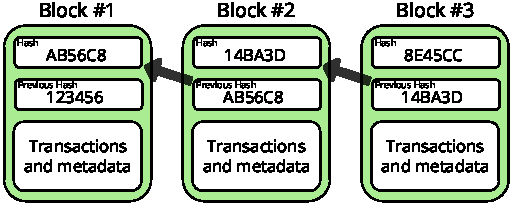
\includegraphics[width=0.7\textwidth]{figures/blockchain.pdf}
  \caption[Blockchain structure]{Blockchain structure showing the chain of blocks.}
  \label{fig:blockchainStructure}
\end{figure}

Blockchains are typically maintained by a \gls{p2p} network, where each participant, referred to as \textit{node}, stores a copy of the blockchain. This decentralized replication ensures data availability, fault tolerance, and security. Nodes follow a consensus protocol, which defines the rules by which transactions are validated and blocks are added to the chain. 

The first blockchain was introduced in 2008 by Satoshi Nakamoto, the pseudonymous creator (or group of creators) of Bitcoin \cite{nakamoto2008bitcoin}. It continues to function as the public ledger for all \acrlong{btc} transactions, effectively solving the \gls{double-spending} problem without the need for a centralized authority. Another widely known blockchain is \acrfull{eth}, which operates alongside its native cryptocurrency, Ether.

%%%%%%%%%%%%%%%%%%%%%%%%%%%%%%%%%%%%%%%%%%%%%%%%%%%%%%%%%%%%%%%%%%
% ETHEREUM
%%%%%%%%%%%%%%%%%%%%%%%%%%%%%%%%%%%%%%%%%%%%%%%%%%%%%%%%%%%%%%%%%%
\section{Ethereum}
\acrlong{eth} was launched in 2015 based on an idea of Vitalik Buterin \cite{buterin2014next}\cite{wood2014ethereum}. Buterin's vision was to enable the deployment of \acrfull{dapp}, programs that run autonomously on a blockchain without relying on external, centralized infrastructure. To realize this vision, he and his collaborators created the \acrfull{evm}, a decentralized virtual machine that executes transactions. In contrast to \acrlong{btc}'s limited instruction set, the \acrshort{evm} supports a broad range of operations, including loops and conditional statements. This flexibility makes it possible to develop \textit{smart contracts}, which are programs containing both code and data that execute on the \acrlong{eth} blockchain.

When users perform on-chain operations, such as sending cryptocurrency or invoking a smart contract function, they consume computational resources. To compensate nodes for providing these resources and to prevent abuse (for example, infinite loops), Ethereum measures resource usage in units called \textit{gas}. Each individual operation requires a specific amount of gas, and the total \textit{gas fee} for a transaction is calculated by multiplying the gas used by the current \textit{gas price}. Because gas is paid in Ether, the cost of executing an operation varies with the market value of Ether.

Users hold Ethers and pay transaction fees via \acrfull{eoa}, which can initiate transactions and serve as the interface between users and the blockchain. An \acrshort{eoa} is derived from a private key, which is also required to cryptographically sign transactions. The other account type in Ethereum is the \textit{contract account}, which corresponds to a deployed smart contract. Contract accounts can hold cryptocurrency but cannot initiate transactions on their own; they can only send transactions in response to receiving one. Both contract accounts and \acrshort{eoa}s are publicly referenced by their address, which serves as the identifier used to send funds or invoke contract functions.

Due to its versatility and the wide range of operations it supports, \acrlong{eth} has become the foundation for numerous Layer 2 solutions \cite{sguanci2021layer2blockchainscaling} over time. Layer 2 solutions are protocols built on-top of the main blockchain (Layer 1) to provide additional features, such as an increased transaction throughput or reduced fees. The core idea behind these solutions is to process transactions off-chain and periodically submitting a summary about them on the Layer 1 chain. Some notable examples of \acrshort{eth} Layer 2 solutions are:

\begin{itemize}
    \item \textit{Polygon}\footnote{\url{https://polygon.technology}}, which offers faster and cheaper transactions compared to the \acrlong{eth} main network.
    \item \textit{Arbitrum}\footnote{\url{https://arbitrum.io}} \cite{kalodner2018arbitrum}, that enhances scalability while preserving compatibility with Ethereum smart contracts.
    \item \textit{ZKsync}\footnote{\url{https://www.zksync.io}}, a solution that ensures high security and fast finality through the use of validity proofs.
    \item \textit{Optimism}\footnote{\url{https://www.optimism.io}}, which prioritizes simplicity and close integration with the Ethereum ecosystem.
    \item \textit{Starknet}\footnote{\url{https://www.starknet.io}}, that introduces its own high-performance language, Cairo\footnote{\url{https://www.cairo-lang.org/}}.
\end{itemize}

%%%%%%%%%%%%%%%%%%%%%%%%%%%%%%%%%%%%%%%%%%%%%%%%%%%%%%%%%%%%%%%%%%
% DECENTRALIZE STORAGE
%%%%%%%%%%%%%%%%%%%%%%%%%%%%%%%%%%%%%%%%%%%%%%%%%%%%%%%%%%%%%%%%%%
\section{Decentralized Storage}
Since blockchain operations consume gas, and gas costs are significantly higher than those in traditional Web 2.0 solutions, especially for storage \cite{surya2024designdecentralizedidentity}, \acrshort{dapp}s often rely on decentralized storage solutions to handle large amounts of data and high-volume files \cite{ray2023web3}\cite{muhle2018survey}. These solutions distribute data across the nodes in the network, in contrast to traditional storage approaches that depends on centralized data centres.

One widely adopted decentralized storage system is \acrfull{ipfs} \cite{benet2014ipfscontentaddressed}, a protocol built on a \gls{p2p} network architecture, similar to blockchains. When users upload a file to \acrshort{ipfs}, it is assigned a unique identifier called a \acrfull{cid}, which corresponds to the \gls{hash} of the file's content \cite{erikflorian2022ipfsandfrineds}. Files can be replicated across multiple nodes to enhance availability and security.  To retrieve a file, users must use its \acrshort{cid} to locate and access the nodes storing it. This content-addressed design ensures file integrity and verifiability, as any change to the file would produce a new \acrshort{cid}.